
\section{Definition of compensators}

\begin{frame}
	\frametitle{Lead Compensator vs Lag Compensator}
	\begin{block}{Schematical representation}
		\begin{figure}
			\centering
			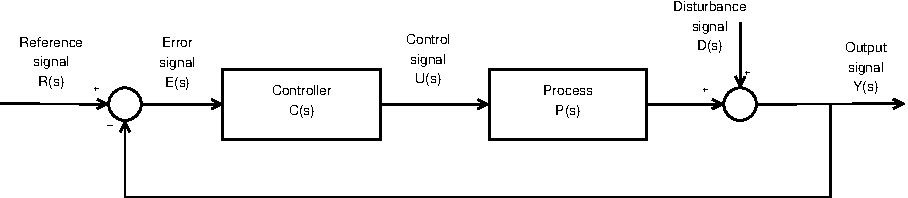
\includegraphics[width=1\linewidth]{Closed-Loop}
		\end{figure}
	\end{block}
	\begin{block}{Transfer functions}
		Lead compensator : 
		$C(s) = K.\frac{s + \frac{1}{\tau}}{s + \frac{1}{\alpha\tau}}$ with $0 \textless  \alpha  \textless  1$ \\
		Lag compensator : 
		$C(s) = K.\frac{s + \frac{1}{\tau}}{s + \frac{1}{\beta\tau}}$ with $\beta  \textgreater  1$
	\end{block}
\end{frame}

\begin{frame}
\frametitle{Lead Compensator vs Lag Compensator: zeros and poles}
\begin{block}{Transfer functions}
	Lead compensator : 
	$C(s) = K.\frac{s + \frac{1}{\tau}}{s + \frac{1}{\alpha\tau}}$ with $0 \textless  \alpha  \textless  1$ \\
	Lag compensator : 
	$C(s) = K.\frac{s + \frac{1}{\tau}}{s + \frac{1}{\beta\tau}}$ with $\beta  \textgreater  1$
\end{block}
\begin{block}{Zeros and poles}
	Zeros: $s = -\frac{1}{\tau}$ \\
	Poles: $s = -\frac{1}{\alpha\tau}$ or $s = -\frac{1}{\beta\tau}$ \\
	For lead compensators the pole lies more to the left in the complex plane than the zero and vice versa for lag compensators.
\end{block}
\end{frame}

\section{Lead compensators}

\begin{frame}
	\frametitle{Transfer function and impact}
	\begin{block}{Impact}
		$C(s) = K.\frac{s + \frac{1}{\tau}}{s + \frac{1}{\alpha\tau}}$ with $0 \textless  \alpha  \textless  1$
		\begin{figure}
			\centering
			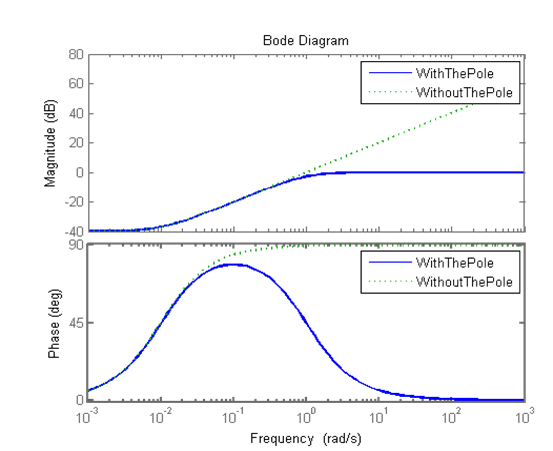
\includegraphics[width=0.5
			\linewidth]{leadcompensator1}
		\end{figure}
	\end{block}
\end{frame}

\begin{frame}	
	\frametitle{Lead compensators}
	\begin{block}{Determination of $\alpha$}
		Use polar plot of 
		$\frac{\alpha.(j\omega\tau + 1)}{j\omega\alpha\tau + 1}$	
		\begin{figure}
			\centering
			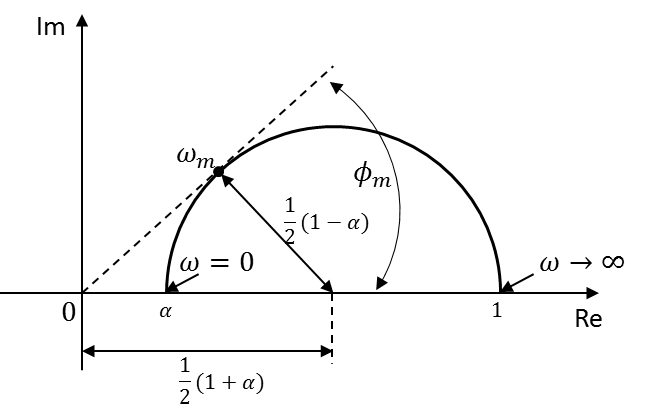
\includegraphics[width=0.5
			\linewidth]{leadcompalphabepalen}
		\end{figure}
		$\sin\phi_m = \frac{\frac{1}{2}.(1 - \alpha)}{\frac{1}{2}.(1 + \alpha)} = \frac{1 - \alpha}{1 + \alpha} \Rightarrow \alpha = \frac{1 - \sin\phi_m}{1 + \sin\phi_m}$ \\
		This relation relates the maximum phase-lead angle and the value of $\alpha$. 
	\end{block}
\end{frame}

\begin{frame}
	\frametitle{Lead compensators}
	\begin{block}{Determination of $\alpha$}
	The figure shows the phase lead in function of $\alpha$. Attention: the phase lead is in radians!
	\begin{figure}
		\centering
		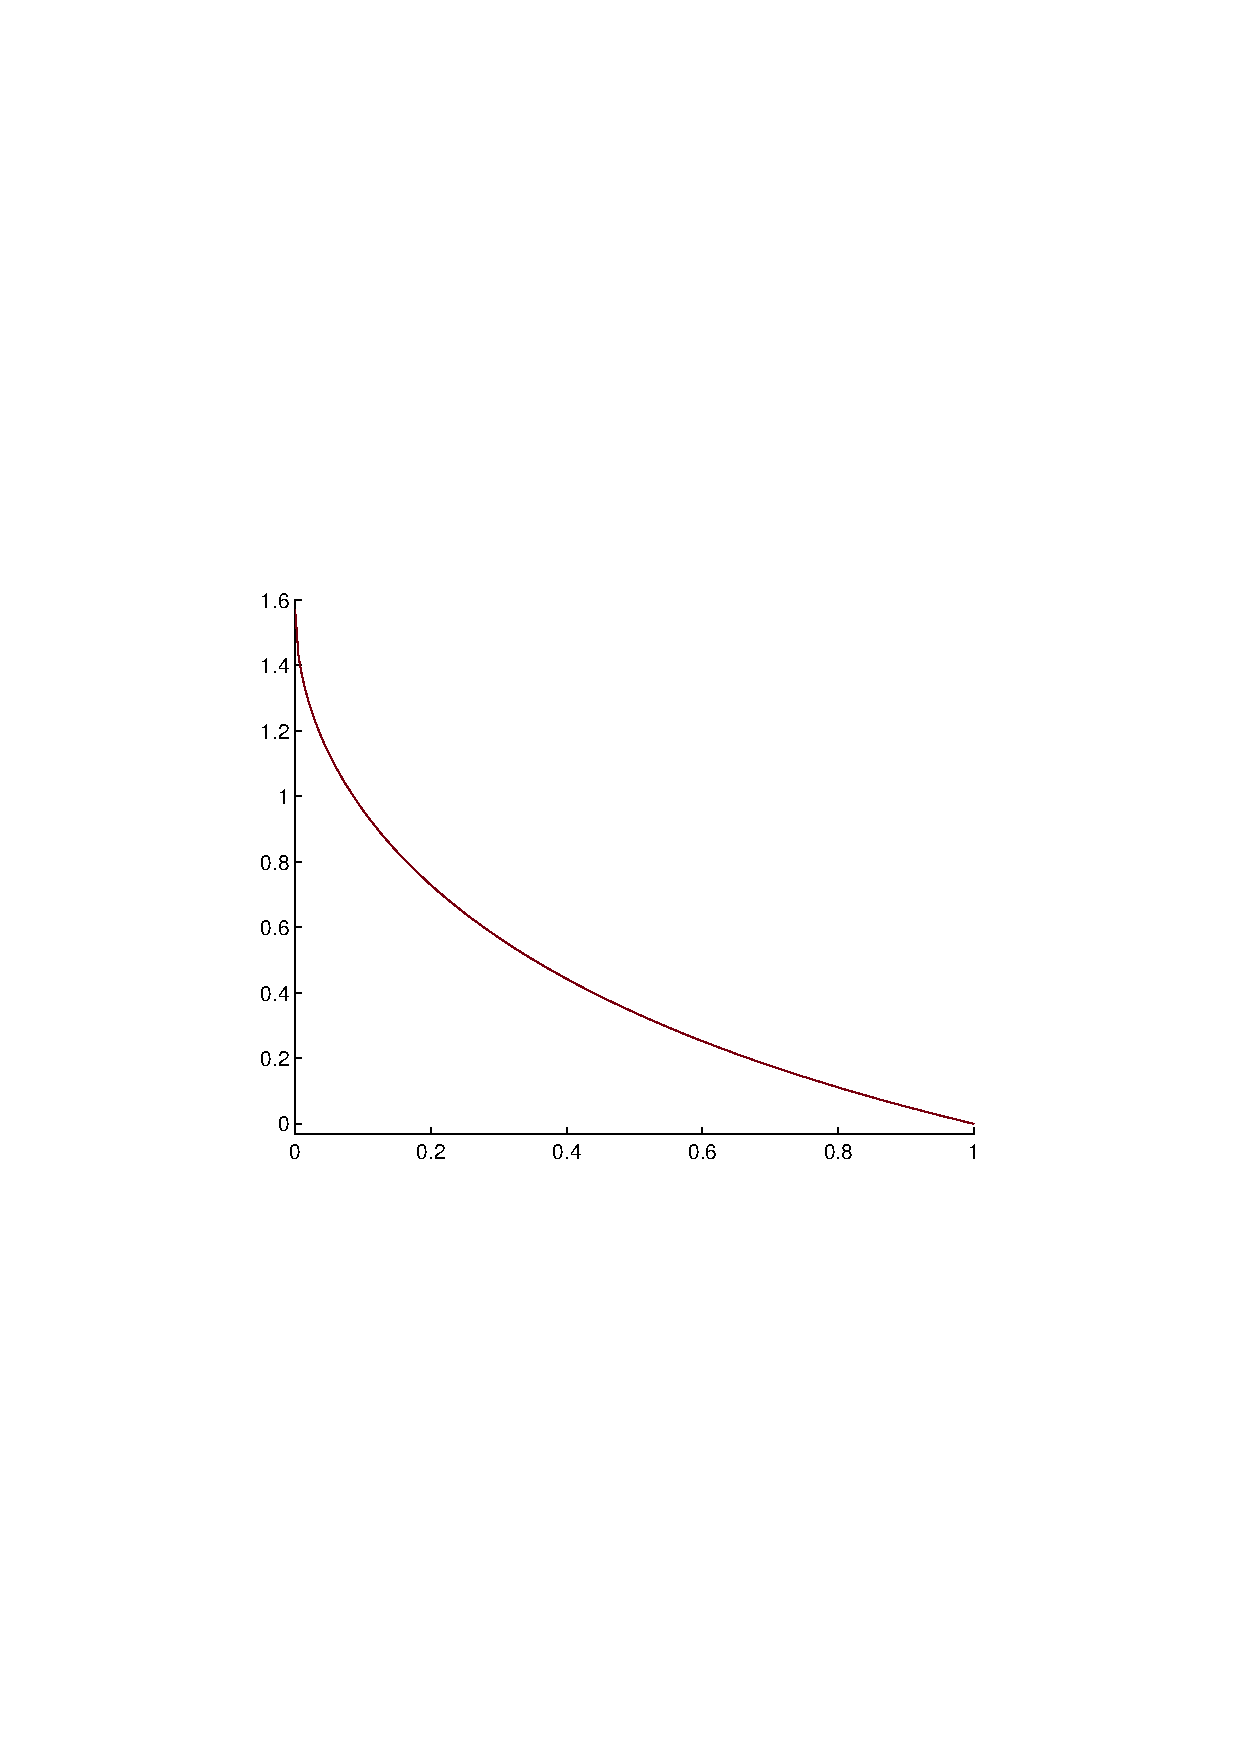
\includegraphics[width=0.5
		\linewidth]{alphavsphi}
	\end{figure}
	Usually, $\alpha \geqslant 0.05 \Rightarrow$ maximum phase lead about $65\,^{\circ}$.
	\end{block}
\end{frame}

\begin{frame}
\frametitle{Lead compensators}
	\begin{block}{Determination of $\tau$}
		\begin{figure}
			\centering
			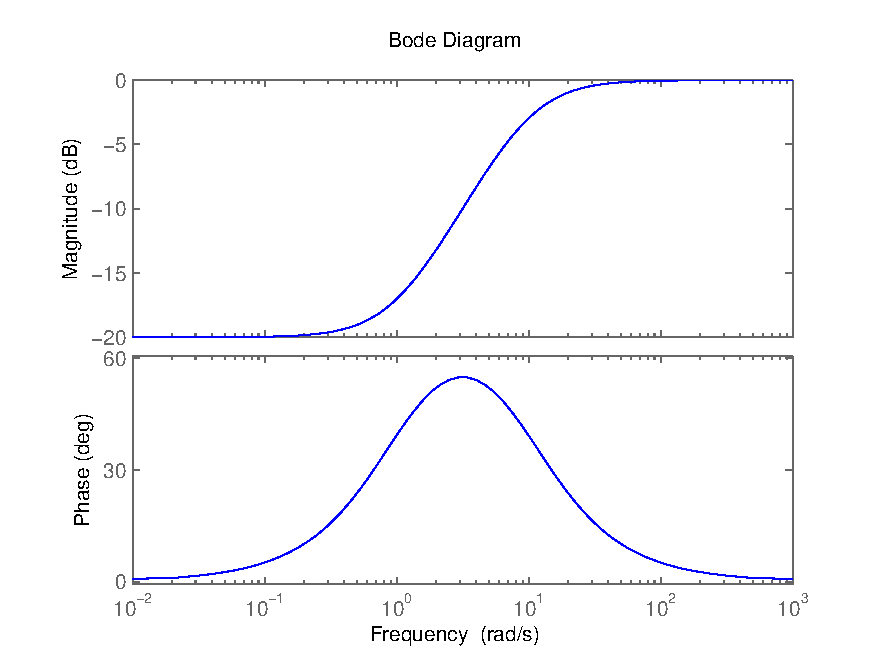
\includegraphics[width=0.5
			\linewidth]{bodelead}
		\end{figure}
		The tangent point $\omega_m$ is the geometric mean of the two corner frequencies, so
		$ \log \omega_m = \frac{1}{2}(\log \frac{1}{\tau} + \log \frac{1}{\alpha\tau})$ with $\tau = \frac{1}{\omega}$
		\\ $\Rightarrow \omega_m = \frac{1}{\sqrt{\alpha}\tau}$. \\
		The lead compensator is a high-pass filter.
	\end{block}
\end{frame}

\begin{frame}
\frametitle{Lead compensators}
\begin{block}{Impact}
	\begin{itemize}
	\item They push the pole of the closed loop system to the left.
	\begin{itemize}
	\item Stabilisation of the system (see root locus)
	\item Increase response speed (lead compensator will stimulate some larger frequencies)
	\end{itemize}
	\item Increase of the phase margin: the phase of the lead compensator is positive for every frequency, and will hence only increase the phase.
	\item Thanks to the presence of a pole, the high frequencies (where most of the unwanted noise is located) are less amplified. Again, a lead compensator is a high-pass filter.
	
	\end{itemize}
\end{block}
\end{frame}

\begin{frame}
\frametitle{Lead compensators}
\begin{block}{Design with Bode plots}
	\begin{itemize}
		\item Design process: tuning of the phase margin, with as a surplus (because we will have one extra degree of freedom) the tuning of the steady state error.
		\item Compensate for the excessive phase lag that is a result of the components of P(s).
		\item Increase in phase at gain crossover frequency (GCF) if GCF is around pole and zero of the lead compensator.
		\item Gain is impacted by the lead compensator: the GCF of P(s).C(s) is not equal to the GCF of P(s).
	\end{itemize}		
\end{block}
\end{frame}

\begin{frame}
	\frametitle{Lead compensators}
	\begin{block}{Design}
		\begin{itemize}
			\item Required increase in phase gain: $\phi$
			\item To compensate for increase GCF due to 
			$C(s) \Rightarrow \phi_m = \phi + 5\,^{\circ}$. This will be needed to determinate $\alpha$ and $\tau$
			\item K will be used to tune the steady state error.
		\end{itemize}		
	\end{block}
\end{frame}


\begin{frame}
\frametitle{Lead compensators}
\begin{block}{Determination of the tangent point}
	Use the gain crossover frequency of P(s)C(s) as $\omega_m$: \\
	$\mid P(j\omega_m)C(j\omega_m) \mid = 1$ \\
	$\mid P(j\omega_m) \mid K \frac{\sqrt{\frac{1}{\alpha\tau^2} + \frac{1}{\tau^2}}}{\sqrt{\frac{1}{\alpha\tau^2} + \frac{1}{\alpha^2\tau^2}}} = \mid P(j\omega_m) \mid K \sqrt{\alpha} = 1$ \\
	$20\log \mid P(j\omega_m) \mid = -20\log (K\sqrt{\alpha})$ \\
	The value of the tangent point $\omega_m$ can be determined from P(s)'s Bode plot, if you know K (the last freedom).
\end{block}
\end{frame}	

\begin{frame}
\frametitle{Lead compensators}
\begin{block}{Determination of K}
	\begin{itemize}
		\item Remember the steady state error for references of the shape: $\frac{At^n\epsilon(\tau)}{n!}$ with $\epsilon(t)$ the step function.
		\item We found the error constants $K_p$, $K_v$ and $K_a$ as measures for the steady state error for a proportional (n=0), linear (n=1) and accelerating (n=2) reference.
		\item These error constants can be used to find proper values of K: 
		$\lim_{s \to 0} K \frac{s + \frac{1}{\tau}}{s + \frac{1}{\alpha\tau}}s^nP(s) = K\alpha \lim_{s \to 0}s^nP(s)$
	\end{itemize}
\end{block}
\end{frame}

\begin{frame}
	\frametitle{Lead Compensation Techniques Based on the Frequency-Response Approach}
	\begin{block}{Step 1}
	Find $K\alpha$ from your steady-state requirement.
	\end{block}
	\begin{block}{Step 2}
	Determine $\phi$, the amount with which you want to increase the PM; if the PM is OK, you don’t need a lead compensator; a proportional controller with gain $K\alpha$ suffices.
	\end{block}
	\begin{block}{Step 3}
	Add $5\,^{\circ}$, to get $\phi_m = \phi + 5\,^{\circ}$ (if $\phi_m > 5\,^{\circ}$, you will need more than one lead compensator). The addition of the lead compensator shifts the gain crossover frequency to the right and decreases the
	phase margin.
	\end{block}
\end{frame}

\begin{frame}
	\frametitle{Lead Compensation Techniques Based on the Frequency-Response Approach}
	\begin{block}{Step 4}
	You will find $\alpha$ from this $\phi_m$: $\alpha = \frac{1 - \sin \phi_m}{1 + \sin \phi_m}$ and hence also K (see step 1). 
	\end{block}
	\begin{block}{Step 5}
		Find the desired $\omega_m$ by looking at the Bode plot of P(s) and finding the frequency at which the gain equals $-20 \log (K\sqrt{\alpha})$ dB.
	\end{block}
	\begin{block}{Step 6}
	Find $\tau$ as $\frac{1}{\sqrt{\alpha}\omega_m}$.
	\end{block}
\end{frame}

\begin{frame}
	\frametitle{Lead Compensation Techniques Based on the Frequency-Response Approach}
	\begin{block}{Step 7}
		Verify if the system works as asked.
		Check the gain margin to be sure it is satisfactory. If not, repeat the design process
		by modifying the pole-zero location of the compensator until a satisfactory result
		is obtained.
	\end{block}
\end{frame}

\begin{frame}
\frametitle{Example}
\begin{block}{Example}
	Given the system $P(s) = \frac{4}{s(s+2)}$. We want a phase margin of at least $50\,^{\circ}$ and a steady state error for slope reference of maximal $\frac{A}{20}$.
	\begin{figure}
		\centering
		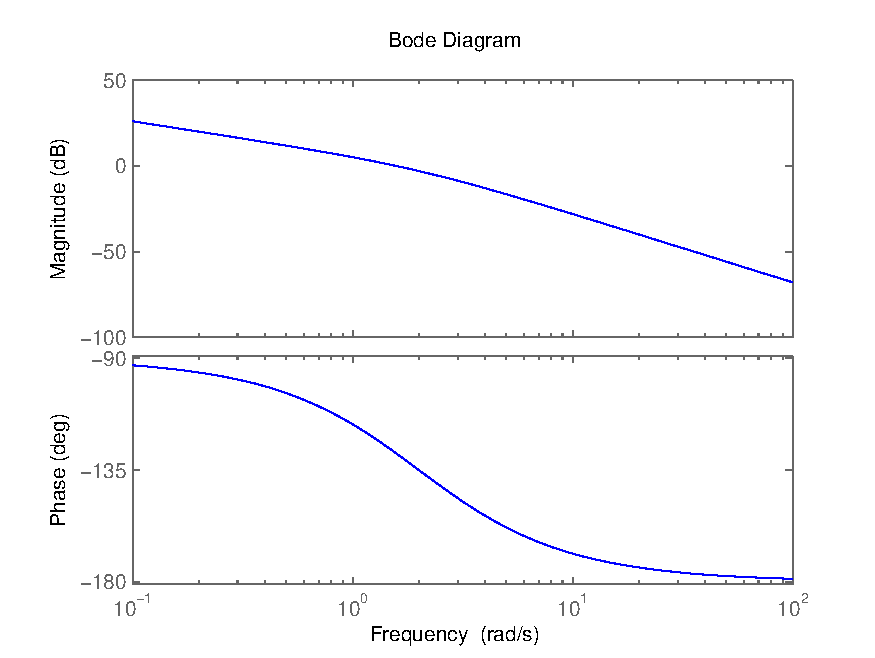
\includegraphics[width=0.5
		\linewidth]{bodeexamplelead}
	\end{figure}
\end{block}
\end{frame}

\begin{frame}
\frametitle{Example}
\begin{block}{Step 1}
Steady-state requirement: $K_v = \frac{20}{s}$ \\
So, $\lim_{s \to 0} sP(s)C(s) = \lim_{s \to 0} s\frac{s}{s(s+2)}K\alpha = 2K\alpha = 20$. \\
$\Rightarrow K\alpha = 10$
\end{block}
\begin{block}{Step 2}
Phase margin of $K\alpha P(s) = 18\,^{\circ}$ (see phase diagram) \\
Calculation of phase margin without phase diagram: \\
We need the frequency where the magnitude is 0 dB. \\So, $20\log \mid K\alpha P(s) \mid = 0$
$\Rightarrow \mid K\alpha P(s) \mid = 1$
$\Rightarrow \mid P(s) \mid = 0.1$ \\
When substituting $s = j\omega$ and calculating the modulus of the complex number at the left side, the equation becomes: \\
$\frac{-4\omega}{\omega (4 + \omega^2)}^2 + \frac{-8}{\omega (4 + \omega^2)}^2 = 0.01$.

\end{block}
\end{frame}

\begin{frame}
	\frametitle{Example}
\begin{block}{Step 2 continued}
This equation has just one real positive solution in $\omega$, $\omega = 6.168$.\\
Now, you have the right frequency. You find the phase margin by calculating the difference between $-180\,^{\circ}$ and the phase of $K\alpha P(6.168j)$.\\ 
We want a phase margin of at least $50\,^{\circ}$
$\Rightarrow \phi = 32\,^{\circ}$
\end{block}
\begin{block}{Step 3}
	$\phi_m = \phi + 5\,^{\circ} = 37\,^{\circ}$
\end{block}
\end{frame}

\begin{frame}
	\frametitle{Example}
	\begin{block}{Step 4}
	 $\alpha = \frac{1 - \sin \phi_m}{1 + \sin \phi_m} = 0.24$ \\
	 From step 1, we know that $K = \frac{\alpha}{10} = 42$
	\end{block}
	\begin{block}{Step 5}
	Find $\omega_m$, the frequency at which the gain is $-20\log(K\sqrt{\alpha})$ dB. 
	$GCF(P(s)K\sqrt{\alpha}) = GCF(P(s)C(s)) \Rightarrow \omega_m = 9 \frac{rad}{s}$ \\
	(see Bode diagram next slide)
	\end{block}
	\begin{block}{Step 6}
	$\tau = \frac{1}{\omega_m\sqrt{\alpha}} = 0.23$
	\end{block}
\end{frame}

\begin{frame}
\frametitle{Example}
\begin{figure}
	\centering
	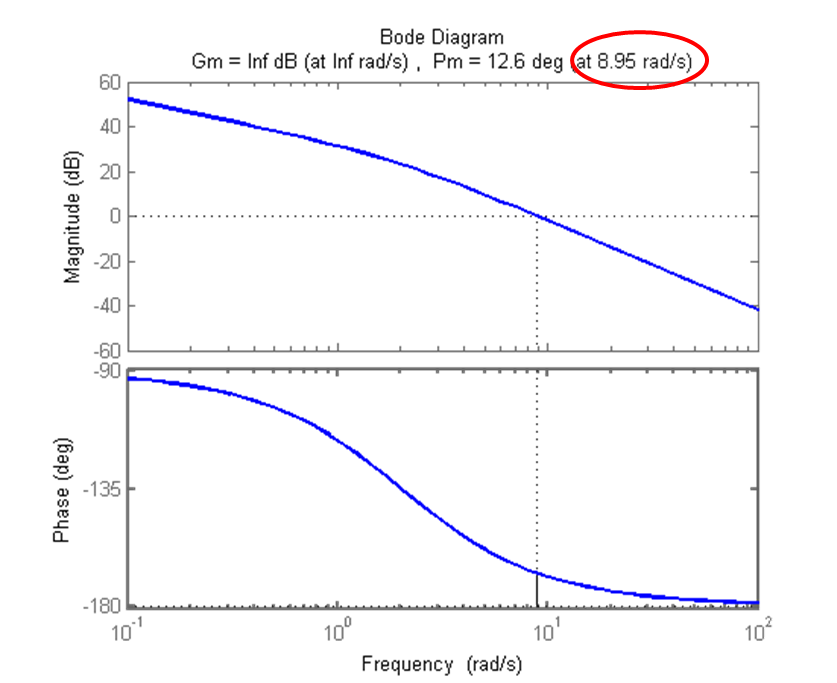
\includegraphics[width=0.7
	\linewidth]{exampleleadstep6}
\end{figure}
\end{frame}

\begin{frame}
	\frametitle{Example}
	\begin{block}{Step 7}
	We verify whether or not our solution is correct. We ask the Bode diagram of $K \frac{4}{s(s+2)} \frac{s+\frac{1}{\tau}}{s+\frac{1}{\alpha\tau}}$ with $\alpha$, $\tau$ and K the results of our calculations. (see next slide) \\
	We see that: 
	\begin{itemize}
		\item the phase margin is indeed more than $32\,^{\circ}$ 
		\item the new tangent point is indeed about $9\frac{rad}{s}$
	\end{itemize} 
	\end{block}
\end{frame}

\begin{frame}
\frametitle{Example}
\begin{figure}
	\centering
	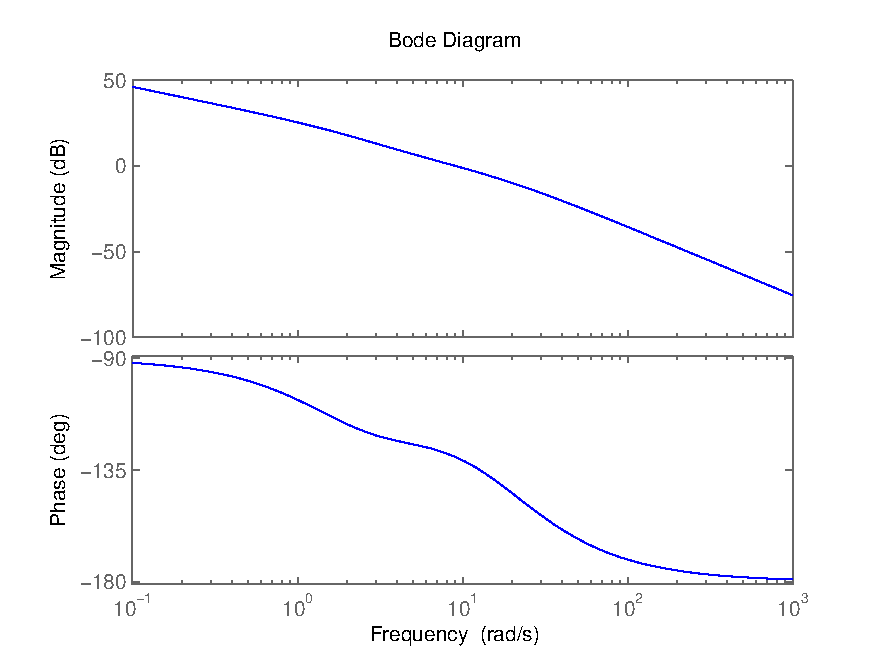
\includegraphics[width=0.7
	\linewidth]{bodesolutionexamplelead}
\end{figure}
\end{frame}

\begin{frame}
	\frametitle{Example}
	\begin{block}{Comparing compensated system vs non-compensated system}
	Blue: non-compensated system \\
	Green: compensated system
	\begin{figure}
		\centering
		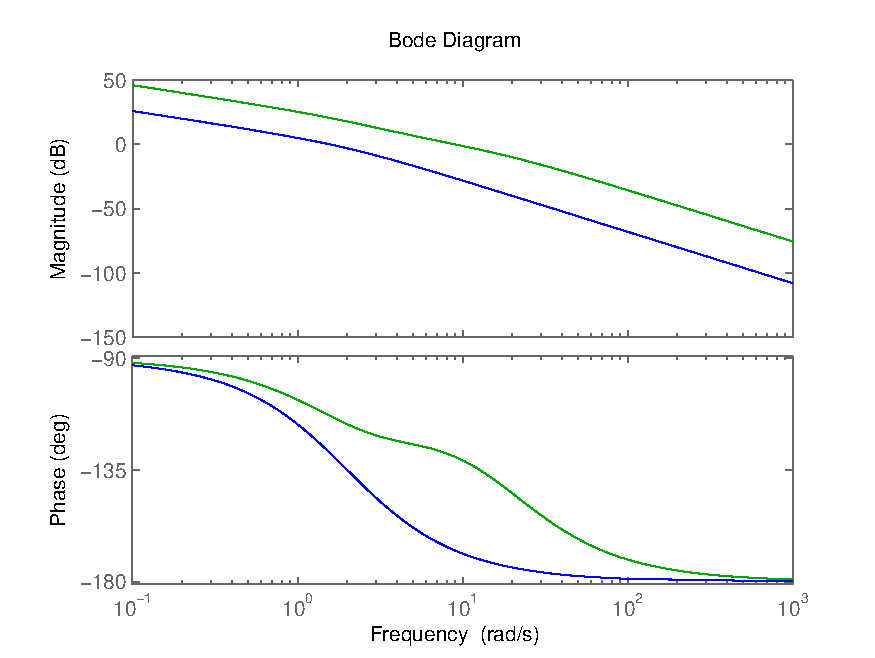
\includegraphics[width=0.5
		\linewidth]{bodesolutionexampleleadcomparing}
	\end{figure}
	\end{block}
\end{frame}

\begin{frame}
\frametitle{Summary lead compensators}
\begin{block}{Evaluation of impact}
\begin{itemize}
	\item Pushing the poles to the left: this is not directly visible here, but is linked to the increased band width.
	\item The increase in bandwidth (this is linked to the response speed) and the increase in the phase margin were apparent in the Bode plot of P(s)C(s).
	\item A (small) decrease in the steady-state error occurs, since we designed it as such. \\
	Why small? The steady-state error decreases when the DC gain gets larger, but a lead compensator’s impact on the gain is not really built to increase the DC gain, the shape of a lag compensator is much more fit for this.
\end{itemize}
\end{block}
\end{frame}

\begin{frame}
	\frametitle{Summary lead compensators}
	\begin{block}{Design with root locus}
	Design lead compensators with root locus for time-domain quantities  - use dominant pole locations to fulfill overshoot, rise time, settling time, damping ratio, … requirements.
	\end{block}
\end{frame}

\section{Lag compensators}

\begin{frame}
	\frametitle{Lag compensators}
	\begin{block}{Transfer function}
		$C(s) = K.\frac{s + \frac{1}{\tau}}{s + \frac{1}{\beta\tau}}$ with $\beta  \textgreater  1$
	\end{block}
	\begin{block}{Bode Diagram}
		Example with K = 1 and $\beta$ = 10 (see next slide) \\ 
		Magnitude of the lag compensator: 
		\begin{itemize}
			\item becomes 10 (= 20 dB) for small frequencies
			\item becomes unity (= 0 dB) for high frequencies
		\end{itemize}
		$\Rightarrow$ Lag compensator is low-pass filter.
		
	\end{block}
\end{frame}

\begin{frame}
\frametitle{Lag compensators}
\begin{block}{Bode Diagram of example}
	\begin{figure}
		\centering
		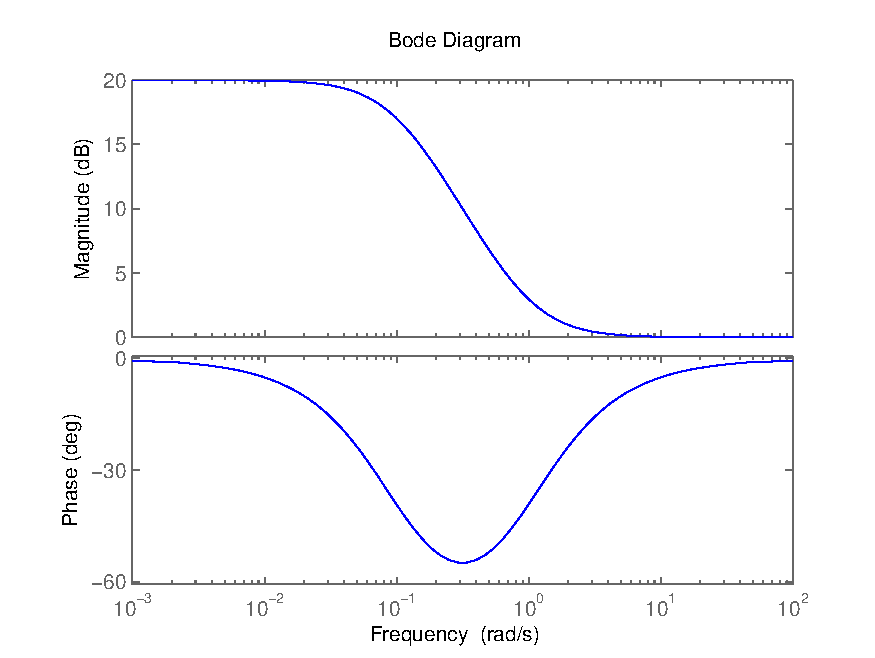
\includegraphics[width=0.5
		\linewidth]{bodelagislowpass}
	\end{figure}
\end{block}
\end{frame}

\begin{frame}
\frametitle{Lag compensators}
\begin{block}{Impact of lag compensators: Bode diagram}
	Blue: non-compensated system \\
	Green: compensated system
	\begin{figure}
		\centering
		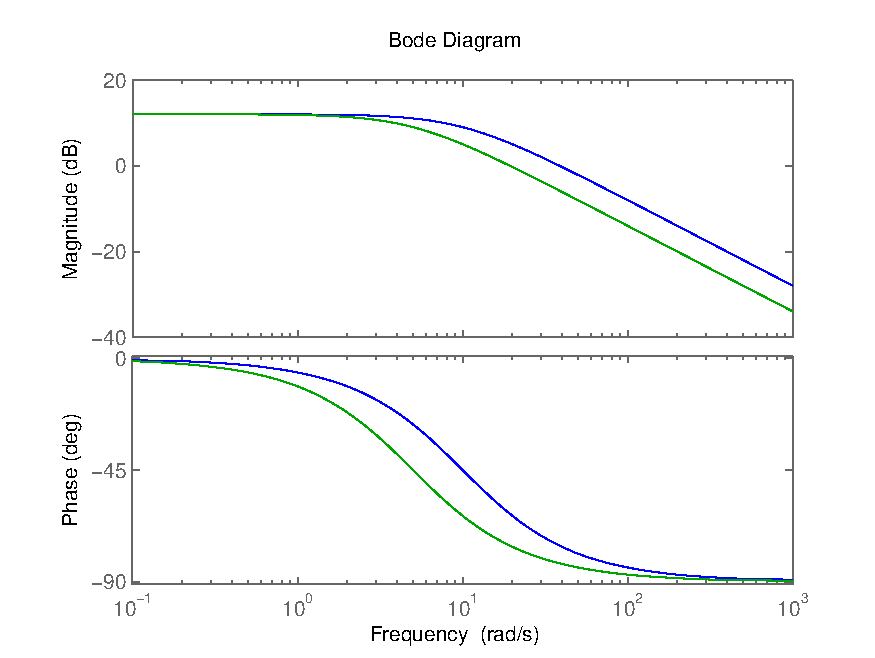
\includegraphics[width=0.5
		\linewidth]{bodelagimpact}
	\end{figure}
\end{block}
\end{frame}

\begin{frame}
	\frametitle{Lag compensators}
	\begin{block}{Impact of lag compensators: Bode diagram}
	\begin{itemize}
		\item Lead compensators: increase the stability and tune the steady-state error by increasing the phase at the crossover frequency.
		\item Impact lag compensator = lead compensator, but different approach!
		By decreasing the gain, the gain crossover frequency comes down to a frequency at which the corresponding phase is higher.
		
	\end{itemize}
	\end{block}
\end{frame}

\begin{frame}
	\frametitle{Lag compensators}
	\begin{block}{Impact of lag compensators}
		Large difference between lead and lag: their effect on the bandwidth of the system and hence on its speed of response.
		\begin{itemize}
			\item A lead compensator increases the bandwidth/speed of response 
			\begin{itemize} 
			\item good if you want the system to react fast
			\end{itemize}
			\item A lag compensator decreases the bandwidth/speed of response 
			\begin{itemize}
			\item good if your model if bad at high frequencies
			\item good to reduce the impact of (mostly high-frequency) noise 
			\end{itemize}
		\end{itemize}
	\end{block}
\end{frame}

\begin{frame}
\frametitle{Lag compensators}
\begin{block}{Design with Bode plots}
We have three degrees of freedom:
\begin{itemize}
	\item to have a sufficient drop in gain
	\item to push the drop in the phase to lower frequencies (that way we can use $\measuredangle P(s)$ as an approximation of $\measuredangle P(s)C(s)$ reliably to some extent
	\item to tune the steady state error
\end{itemize}
		
\end{block}
\end{frame}

\begin{frame}
	\frametitle{Lag compensators}
	\begin{block}{Design with Bode plots}
		\begin{itemize}
		\item Increase of phase margin $\Rightarrow$ decrease of the magnitude at some higher frequencies 
		\item Decrease of the steady state error $\Rightarrow$ increase of the magnitude at DC
		\end{itemize}
		A lag compensator can realize both conditions.
		\begin{itemize}
			\item At DC value, the gain becomes: $\lim_{s \to 0} K\frac{s + \frac{1}{\tau}}{s + \frac{1}{\beta\tau}} = K\beta$
			\item At high frequencies, the gain becomes:
			$\lim_{s \to \infty} K\frac{s + \frac{1}{\tau}}{s + \frac{1}{\beta\tau}} = K$ 
		\end{itemize}
	\end{block}
\end{frame}

\begin{frame}
	\frametitle{Lag compensators}
	\begin{block}{Design with Bode plots}
	K has to be such that the drop in magnitude is sufficient, the value of $\beta$ has make the steady state error decrease enough and the value of $\tau$ has to be such that the transfer between from $K\beta$ to $\tau$ occurs at the right frequency.
	\begin{figure}
		\centering
		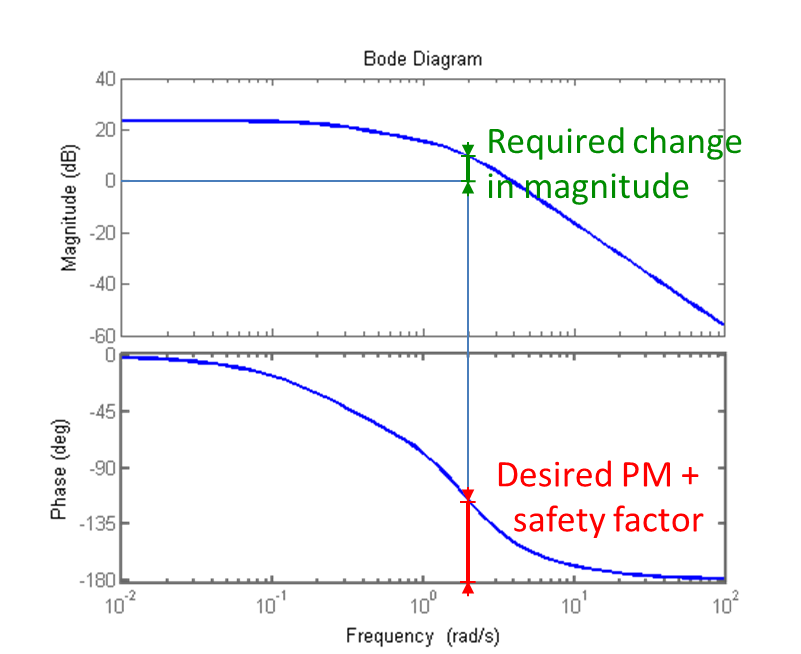
\includegraphics[width=0.5
		\linewidth]{determinationKLagcompensator}
	\end{figure}
	\end{block}
\end{frame}

\begin{frame}
	\frametitle{Lag compensators}
	\begin{block}{Determination of K}
	\begin{itemize}
		\item Easily read from Bode plot (slide before).
		\item Find the frequency ($\omega$) with desired phase margin (+ safety factor), then find the magnitude at that frequency; which is equal to the required change in magnitude (= Q). \\
		$\Rightarrow$ $K = \frac{1}{Q}$ \\
		$\Rightarrow$ Safety factor about $10\,^{\circ}$
		\begin{itemize}
			\item the drop in magnitude will not be complete (this is very marginal)
			\item the lag compensator influences the phase plot
		\end{itemize}
	\end{itemize}
	\end{block}
\end{frame}

\begin{frame}
	\frametitle{Lag compensators}
	\begin{block}{Determination of $\beta$}
	$\Rightarrow$ in a similar way as we found $K\alpha$ for the lead compensator
	\begin{itemize}
	\item Translate steady state error requirement in a requirement on:
	\begin{itemize}
		\item $K_p = \lim_{s \to 0} (P(s)C(s))$
		\item $K_v = \lim_{s \to 0} s(P(s)C(s))$
		\item $K_a = \lim_{s \to 0} s^2(P(s)C(s))$
		\item or another error constant
	\end{itemize}
	\item With this $K_p/K_v/K_a$ and $\lim_{s \to 0} P(s)$, we can determine $\lim_{s \to 0}C(s) = K\beta$
	\end{itemize}
	\end{block}
\end{frame}

\begin{frame}
	\frametitle{Lag compensators}
	\begin{block}{Determination of $\tau$}
	\begin{itemize}
	\item Take $\tau$ large enough such that the magnitude is almost entirely dropped, and the phase drop has almost disappeared.
	\item Take the zero one decade smaller than the frequency ($\omega$) at which P(s) had the desired phase ($-180\,^{\circ}$ + the desired phase margin + a safety factor of $10\,^{\circ}$). The addition of $10\,^{\circ}$ compensates for the phase lag of the lag compensator.
	\item Verify the effect of a single zero at a frequency one decade smaller than $\omega$.
	\begin{itemize}
	\item The drop in magnitude is as good as complete.
	\item The drop in phase cannot be more than $-5.7\,^{\circ}$.
	\end{itemize}
	\end{itemize}
	\end{block}
\end{frame}

\begin{frame}
\frametitle{Lag Compensation Techniques Based on the Frequency-Response Approach}
\begin{block}{Step 1}
	Translate your steady-state requirement into a requirement on $\lim_{s \to 0}C(s) = K\beta$ and verify whether a proportional controller with gain $K\beta$ would suffice.
\end{block}
\begin{block}{Step 2}
	Read $\omega$, the frequency at which the phase margin equals $-180\,^{\circ}$ + "your desired phase margin" + $10\,^{\circ}$, off the Bode diagram. This allows us to compute $\tau = \frac{10}{\omega}$. 
\end{block}
\end{frame}

\begin{frame}
	\frametitle{Lag Compensation Techniques Based on the Frequency-Response Approach}
	\begin{block}{Step 3}
	Read Q, the magnitude at $\omega$ off the Bode plot and determine $K = \frac{1}{Q}$
	\end{block}
	\begin{block}{Step 4}
	We just have calculated K (step 3) and we know $K\beta$ (step 1), so it's possible to determine $\beta$.
	\end{block}
	\begin{block}{Step 5}
		Verify the behavior of the resulting system.
	\end{block}
\end{frame}











